\message{ !name(ch_3.tex)} %%%%%%%%%%%%%%%%%%%%%%%%%%%%%%%%%%%%%%%%%%%%%%%%%%%%%%%%%%%%%%%%%%%%%%%%%%%%%%%%%%%%%%%%%%%%%%%%%%%%%%%%%%%%%%%%%%%%%%%%%%%%%%%%%%%%%%%%%%%%%%%%%%%%%%%%%%%
% This is just an example/guide for you to refer to when submitting manuscripts to Frontiers, it is not mandatory to use Frontiers .cls files nor frontiers.tex  %
% This will only generate the Manuscript, the final article will be typeset by Frontiers after acceptance.   
%                                              %
%                                                                                                                                                         %
% When submitting your files, remember to upload this *tex file, the pdf generated with it, the *bib file (if bibliography is not within the *tex) and all the figures.
%%%%%%%%%%%%%%%%%%%%%%%%%%%%%%%%%%%%%%%%%%%%%%%%%%%%%%%%%%%%%%%%%%%%%%%%%%%%%%%%%%%%%%%%%%%%%%%%%%%%%%%%%%%%%%%%%%%%%%%%%%%%%%%%%%%%%%%%%%%%%%%%%%%%%%%%%%%

%%% Version 3.3 Generated 2016/11/10 %%%
%%% You will need to have the following packages installed: datetime, fmtcount, etoolbox, fcprefix, which are normally inlcuded in WinEdt. %%%
%%% In http://www.ctan.org/ you can find the packages and how to install them, if necessary. %%%
%%%  NB logo1.jpg is required in the path in order to correctly compile front page header %%%

\documentclass[utf8]{frontiersSCNS} % for Science, Engineering and Humanities and Social Sciences articles
%\documentclass[utf8]{frontiersHLTH} % for Health articles
%\documentclass[utf8]{frontiersFPHY} % for Physics and Applied Mathematics and Statistics articles

%\setcitestyle{square} % for Physics and Applied Mathematics and Statistics articles
\usepackage{url,hyperref,lineno,microtype,subcaption}
\usepackage[onehalfspacing]{setspace}
\usepackage{graphicx}
\usepackage{algorithm}
\usepackage{algorithmic}
\usepackage{multirow}
\usepackage{amsmath}
\usepackage{color}
%\usepackage{natbib}
\usepackage{setspace}

\renewcommand{\algorithmicrequire}{\textbf{输入:}}
\renewcommand{\algorithmicensure}{\textbf{输出:}}

\newenvironment{varalgorithm}[1]
  {\algorithm\renewcommand{\thealgorithm}{#1}}
  {\endalgorithm}


\linenumbers


% Leave a blank line between paragraphs instead of using 


\def\keyFont{\fontsize{8}{11}\helveticabold }
\def\firstAuthorLast{Zhan Peng, Yuping Wang} %use et al only if is more than 1 author
\def\Authors{Zhan Peng$^1$, \, Yuping Wang\,$^{1*}$}
% Affiliations should be keyed to the author's name with superscript numbers and be listed as follows: Laboratory, Institute, Department, Organization, City, State abbreviation (USA, Canada, Australia), and Country (without detailed address information such as city zip codes or street names).
% If one of the authors has a change of address, list the new address below the correspondence details using a superscript symbol and use the same symbol to indicate the author in the author list.
\def\Address{$^1$School of Computer Science and Technology, Xidian
  University, Xi'an, Shanxi, China}
% The Corresponding Author should be marked with an asterisk
% Provide the exact contact address (this time including street name and city zip code) and email of the corresponding author
\def\corrAuthor{}

\def\corrEmail{ywang@xidian.edu.cn}


\begin{document}

\message{ !name(ch_3.tex) !offset(-3) }

\onecolumn
\firstpage{1}

\title[A Novel Graph Model For The MLCS Problem]{\\
  A Novel Efficient Graph Model For The Multiple Longest Common
  Subsequences (MLCS) Problem}

\author[\firstAuthorLast ]{\Authors} %This field will be automatically populated
\address{} %This field will be automatically populated
\correspondance{} %This field will be automatically populated

\extraAuth{}% If there are more than 1 corresponding author, comment this line and uncomment the next one.
%\extraAuth{corresponding Author2  Laboratory X2, Institute X2, Department X2, Organization X2, Street X2, City X2 , State XX2 (only USA, Canada and Australia), Zip Code2, X2 Country X2, email2@uni2.edu}


\chapter{求解最长公共子序列(MLCS)问题的层次化图模型}


\section{引言}
\label{sec:introduction}

度量生物序列间的相似性是生物信息学中的一类基本问题,它们在癌症检
测\cite{Aravanis2017},探寻物种的共同起源\cite{Zvelebil2007}等许多方面具有广泛的
应用。度量序列间相似性最重要手段之一是寻找序列间的最长公共子序列 (Longest Common
Subsequence,简称为LCS), 这已被证实是一类NP难问题\cite{Maier1978}。根据目标序列的
个数,该问题可以被分为两类:(1)寻找两个序列的最长公共子序列被称为最长公共子序
列(LCS)问题;(2) 寻找超过两个序列的最长公共子序列被称为多最长公共子序列(MLCS)问
题。

传统上, 研究工作主要集中于第一类问题。然而近些年来,越来越多的来自生物信息学及其
他领域的应用要求寻找超过两个序列的最长公共子序列(MLCS)。例如,多序列比
对(Multiple Sequence Alignment) 是MLCS问题在生物信息学中最主要的应用之一,该技术
能够重排多个DNA,RNA,或蛋白质序列,找出序列间具有相似性的片段,以此来识别序列间
功能性的,结构性的,或进化性的联系。 MLCS算法同样可以应用到许多其他种类的序列中,
比如在自然语言处理中计算字符串之间的编辑距离,以及应用到许多金融类数据中。目前,
针对这些应用的现有算法大多基于支配点图模型--该类算法将基于目标序列构建支配点有向
无环图(DAG),从而将寻找序列MLCS的问题转化为寻找有向无环图中最长路径的问题。但是由
于这类算法构造DAG的时间/空间开销过大,使其无法应用于多序列或长序列的情形。

本章中,我们提出了一种时空高效的有向无环图模型,被称为“层次化有向无环图”(简称
为Leveled-DAG),同时设计了相应的构建算法。类似于现有(基于支配点的)算法中的有向无
环图的构造方式,Leveled-DAG模型将被逐层地构造,然而,区别于现有算法在构造有向无环
图时需要产生大量节点并将其全部保存在内存中, Leveled-DAG模型会实时地删除那些过时的
节点, 这些节点不会对构造MLCS再产生影响的。 在任意时刻,Leveled-DAG只需保存新产生
的一层节点及部分以前产生的节点,因此,Leveled-DAG的规模比现有算法构造的有向图无环
图小很多,这会极大的减少空间开销。此外,随着构建过程的进行,Leveled-DAG的规模将越
来越小,最终将只包含一个节点(终止节点),而目标序列的MLCS都存储在该节点中从而直接
可得,无序任何额外操作来寻找MLCS,这将节省算法的运行时间, 提高算法效率。 实验结果
证实,Leveled-DAG模型在时间和空间两方面均非常高效,尤其对于大规模或长序列
集,Leveled-DAG模型明显优于现有方法。

本章组织如下: 节介绍了背景知识及相关工作;节详细的介绍了Leveled-DAG模型及其构建
算法;节进行了仿真实验和结果分析;节总结了本章内容。



\section{相关概念}
\label{sec:MM}

首先, 令 $\Sigma$ 表示序列的字符集, 即序列中所出现符号的有限集合. 例如, DNA序列的
字符集是: $\Sigma=\{A, C, G, T\}$.

\textbf{定义 1.} 令 $\Sigma$ 表示序列的字符集,令 $s=c_1c_2...c_n$ 表示长为 $n$
的一个序列,其中每个字符 $c_i\in\Sigma$, $i=1,2,\cdots,n$. 序列 $s$ 中的第 $i$ 个
字符表示为 $s[i]=c_i$. 如果一个序列 $s'$ 是由删除 $s$ 中零个或多个(不一定连续)字
符而得到的,即 $s'=c_{i_1}c_{i_2}...c_{i_k}$ 且满足 $1 \leq i_1<i_2<\cdots<i_k
\leq n$, 则序列 $s'$ 被称为序列 $s$ 的一个长为 $k$ 的子序列。

\textbf{定义 2.} 给定字符集 $\Sigma$ 上的 $d$ 个序列 $s_1, s_2, ..., s_d$, 如果一
个序列 $s'=c_{i_1}c_{i_2}...c_{i_k}$ 满足: (1) 它是 $d$ 个序列中每一个序列的子序
列。 (2) 它是 $d$ 个序列最长的子序列. 则 $s'$ 被称为这 $d$ 个序列的最长公共子序
列(简称为LCS)。

通常, 多个序列的最长公共子序列并不唯一。 例如,给定三个DNA序列 $ACTAGTGC$,
$TGCTAGCA$ 和 $CATGCGAT$, 它们有两个长为4的最长公共子序列,分别
是 $CAGC$ 和 $CTGC$. 所谓的多最长公共子序列(MLCS)问题, 就是要找出三个或多个目标序
列的所有最长公共子序列。

针对MLCS问题,在过去几十年中,许多算法已被提出。根据这些算法所基于的模型,它们可
以被分为两大类:基于动态规划的算法和基于支配点模型的算法。下面将简要介绍这两类方
法。

\subsection{基于动态规划的算法}
\label {sec:Dynamic Programming}

求解MLCS问题的经典方法基于动态规划 \cite{Smith1981}, \cite{Sankoff1972}. 给定$d$
个序列 $s_1,\, s_2,\,...,\, s_d$, 其长度分别为 $n_1,\, n_2,\, ...,\, n_d$, 基于动
态规划的算法将递归的构造一个具有 $n_1 \times n_2 \times ... \times n_d$ 个元素
的“得分矩阵” $T$, 其中元素 $T[i_1,\, i_2,\, ...,\, i_d]$ 记录了前缀序
列 $s_1[1...i_1]$, $s_2[1...i_2]$, ..., $s_d[1...i_d]$ 的最长公共子序列的长
度。 元素 $T[i_1,\, i_2,\, ...,\, i_d]$ 可由以下公式递归计算:

\begin{equation}
  T[i_1,\, i_2,\, ...,\, i_d] =
  \begin{cases}
    0 & \text{if $\exists j(1 \leq j \leq d), i_j = 0$}\\
    T[i_1-1,\, ...,\, i_d-1] + 1  & \text{if $s_1[i_1] = s_2[i_2] =
      ... = s_d[i_d]$}\\
    max(\bar{T}) & \text{otherwise}
  \end{cases}
\end{equation}

其中
$\bar{T} = \{T[i_1-1,\, i_2,\, ...,\, i_d],\, T[i_1,\, i_2-1,\, ...,\, i_d],\,
...,\, T[i_1,\, i_2,\, ...,\, i_d-1]\}$. 一旦得分矩阵 $T$ 构建完成, 目标序列的最
长公共子序列可由 $T$ 的最后一个元素 $T[n_1,\, n_2,\, ...,\, n_d]$ 向其第一个元
素 $T[0,\, 0,\, ...,\, 0]$ 进行反向回溯而得到。 图 \ref{fig:DM} A 显示了两个序
列 $s_1 = ACTAGCTA$ 和 $s_2 = TCAGGTAT$ 的得分矩阵 $T$. 如图\ref{fig:DM} (B) 所
示, 这两个序列的最长公共子序 (分别是 $TAGTA$ 和 $CAGTA$), 可由元素 $T[8,\, 8]$
向元素 $T[0,\, 0]$ 进行回溯而得到。

\begin{figure}[!h]
  \centering
  \includegraphics[height=2in, width=4.5in]{./eps/DM}
  \caption{(A) 两个DNA序列 ACTAGCTA 和 TCAGGTAT 的得分矩阵. (B) 通过得分矩阵构建
    最长公共子序列,其中的阴影元素对应于支配点.}
\label{fig:DM}
\end{figure}

很明显,对于具有相同长度 $n$ 的 $d$ 个序列, 使用基于动态规划的算法求解其MLCS的时
间和空间复杂度均为 $O(n^d)$ \cite{Hsu1984}. 已经有许多算法被提出用于改进基于动态
规划方法的效率, \cite{Hirschberg1977}, \cite{Apostolico1992}, \cite{Masek1980},
\cite{Rick1994}. 然而, 随着 $d$ 和 $n$ 的增加, 所有这些方法的效率仍然无法满足实际
需求。

\subsection{基于支配点的算法}
\label{sec:Dominant Point}

为了减少基于动态规划方法的时空复杂度,许多新方法已被提出,基于支配点图模型的算法
是其中最有效的方法之一。在介绍该方法前首先给出一些基本定义。

\textbf{定义 3.} 给定 $\Sigma$ 上的 $d$ 个序列 $s_1,\, s_2,\, ...,\,
s_d$, 向量 $p = (p_1,\, p_2,\, ...,\, p_d)$ 被称为这 $d$ 个序列的一个匹配点, 如果
其满足 $s_1[p_1] = s_2[p_2] = ... = s_d[p_d] = \delta$, 即 $\delta$ 是位于序
列 $s_i$ 第 $p_i$ ($i=1,2,\cdots,d$) 个位置的公共字符。 匹配点 $p$ 所对应的公共字
符 $\delta$ 表示为 $C(p)$.

\textbf{定义 4.} 给定 $d$ 个序列的两个匹配点 $p = (p_1,\, p_2,\, ...,\,
p_d)$ 和 $q = (q_1,\, q_2,\, ...,\, q_d)$, 我们称: (1) $p = q$ 当且仅当 $p_i =
q_i$ ($1 \leq i \leq d$). (2) $p$ 支配 $q$ 或 $q$ 被 $p$ 支配 (表示为 $p \preceq
q$), 如果对每一个 $i$ ($1 \leq i \leq d$) 都有 $p_i \leq q_i$, 并且存在 $j$
($1 \leq j \leq d$) 使得 $p_j<q_j$. (3) $p$ 强支配 $q$ 或 $q$ 被 $p$ 强支配 (表示
为 $p \prec q$), 如果对每一个 $i$ ($1 \leq i \leq d$) 都有 $p_i < q_i$. (4) $q$
是 $p$ 的一个后继或 $p$ 是 $q$ 的前驱, 如果 $p \prec q$ 并且不存在匹配
点 $r$ 使得 $p \prec r \prec q$ 且 $C(q) = C(r)$.

注意, 一个匹配点最多有 $|\Sigma|$ 个后继, 其中每个后继对应于 $\Sigma$ 中的一个字
符。

\textbf{定义 5.} 匹配点 $p = (p_1,\, p_2,\, ...,\, p_d)$ 所在的层次被定义
为 $L(p) = T[p_1,\, p_2,\, ...,\, p_d]$, 其中 $T$ 是由公式 (1) 计算得到的得分矩
阵。 匹配点 $p$ 被称为一个 $k$-支配点, 当且仅当: (1) $L(p) = k$. (2) 不存在其他匹
配点 $q$ 使得 $L(q) = k$ 且 $q \preceq p$. 所有 $k$-支配点构成了集合 $D^k$.\\

基于支配点模型的方法的动机在于减少动态规划方法的时空复杂度。 其核心思想基于这样的
事实,即只有支配点才能够影响MLCS的构建(如图\ref{fig:DM} B 所示, 阴影元素对应于
支配点)。由于支配点的数量远小于矩阵 $T$ 中的所有元素的数量,而基于支配点模型的方
法将只需计算支配点而非整个矩阵的元素,因此相比动态规划方法极大地降低了时空复杂
度。

基于支配点模型的算法的搜索空间可以被组织为一个有向无环图(DAG): 图中的每一个节点代
表一个匹配点,边 $\langle p,\, q \rangle$ 代表 $q$ 是 $p$ 的一个后继,即 $p
\prec q$ 且 $L(q) = L(p) + 1$. 最初, 图中仅包含一个没有任何入边的源节点 $(0,\,
0,\, ...,\, 0)$ 以及一个没有任何出边的终止节点 $(\infty,\, \infty,\, ...,\,
\infty)$. 接着, 有向无环图将按照如下方式被逐层构造: 首先, 令层次 $k =
0$, 且 $D^0 = \{(0,\, 0,\, ...,\, 0)\}$, 然后,
通过一个正向迭代的过程:$D^k \rightarrow D^{k+1}$, $(k+1)$-支配点集 $D^{k+1}$ 将
基于 $k$-支配点集 $D^k$ 而产生。 具体地, $D^k$ 中的每个节点将会通过产生其所
有 $|\Sigma|$ 个后继而被扩展, 接着通过一个被称为 $Minima$ 的剪枝操作找出所有那些
支配其它节点的支配点,只有这些支配点才被保留下来以构成 $D^{k+1}$. 一旦图中所包含
的所有节点均已被扩展, 整个有向无环图便构造完毕, 图中从源节点到终止节点的一条最长
路径对应于目标序列的一个最长公共子序列, 这样, MLCS 问题便转化为寻找图中从源节点到
终止节点的所有最长路径的问题. 下面将给出一个简单的例子来说明以上过程。

\textbf{例 1.} 基于支配点模型求解序列 $ACTAGCTA$ 和 $TCAGGTAT$ 的最长公共子序列,
如图 \ref{fig:DAG} 所示。

\begin{figure}[!h]
  \centering
  \includegraphics[height=3.8in, width=3.6in]{./eps/DAG}
  \caption{基于支配点模型所构造的序列 $ACTAGCTA$ 和 $TCAGGTAT$ 的有向无环图,图中
    黑色和灰色的节点将被 $Minima$ 剪枝操作删除。}
  \label{fig:DAG}
\end{figure}


\begin{itemize}
\item \textbf{步骤 0}. 产生源节点 $(0,0)$ 和终止节点 $(\infty, \infty)$.
\item \textbf{步骤 1.} 构造图的第一层节点。 对于字符 $A$, 其匹配点 $(1,3)$ 中的两
  个分量分别是 $A$ 在两个输入序列中第一次出现的位置。 这样, 节点 $A(1,3)$ 便是源
  节点在第一层中对应于字符 $A$ 的后继。 类似地, 节点 $C(2,2)$,
  $G(5,4)$ 和 $T(3,1)$ 是源节点分别对应于字符 $C$, $G$ 和 $T$ 的后继。 在第一层的
  这4个节点当中, 通过 \emph{Minima} 剪枝操作找出并删除被支配
  点 $G(5,4)$, 如图 \ref{fig:DAG} 中灰色节点所示。 剩下的3个支配节点构成了图的第
  一层 $D^1=\{A(1,3),C(2,2),T(3,1)\}$.
  
\item \textbf{步骤 2}. 构造图的第二层节点。 对于 $D^1$ 中的每一个节
  点, 比如 $A(1,3)$, 由于匹配点 $(4,7)$ 的分量是继匹配点 $(1,3)$ 之后字符 $A$ 在
  两个序列中第一次出现的位置。 这样, 节点 $A(4,7)$ 便是节点 $A(1, 3)$ 在第二层中
  对应于字符 $A$ 的后继。 类似地, 节点 $T(3,6)$ 和 $G(5,4)$ 是节点 $A(1, 3)$ 在第
  二层中分别对应于字符 $T$ 和 $G$ 的后继。 以此类推, 第一层中的节点 $C(2,2)$ 可以
  产生3个第二层中的后继节点: $A(4,3)$, $G(5,3)$ 和 $T(3,6)$,第一层中的节
  点 $T(3,1)$ 可以产生4个第二层中的后继节点: $A(4,3)$, $C(6,2)$,
  $G(5,4)$ 和 $T(7,6)$。 注意, 有些节点会被重复产生。 在新产生的第二层的10个节点
  中, 通过剪枝操作 \emph{Minima} 找到并删除重复节点 $A(4,3)$, $G(5,4)$ (会被删除
  两次) 和 $T(3,6)$, 如图第二层中的黑色节点所示。 同样, 通过 \emph{Minima} 操作
  找到并删除被支配节点 $(4, 7)$, $(5, 4)$ 和 $(7, 6)$ 如图第二层中的灰色节点所
  示。 剩余的支配点构成了图的第二层 $D^2=\{T(3, 6),\; A(4, 3),\;$ $C(6,2)\}$。 注
  意, 如果一个节点没有任何后继,那么令终止节点为其唯一后继。
\item \textbf{步骤 3}. 逐层重复以上步骤,直到有向无环图构造完毕,即图中所有节
  点(除了终止节点)均已被扩展。
  
\end{itemize}

从以上例子可以看出,基于支配点模型的方法有以下两个缺陷:
\begin{enumerate}
\item 每层中会产生大量重复的,被支配的冗余节点,它们将消耗大量的存储空间。
\item 找出并删除冗余节点的剪枝操作需要对大量的 $d$ 维向量进行逐对比较,每次比较又
  需要 $d$ 次整数比较,当 $d$ 较大时,对每一层进行剪枝操作将会变得极其耗时。
\end{enumerate}

\cite{Hunt1977} 首次提出了针对两个序列的基于支配点的算法,其时间复杂度
为 $O((r+n)logn)$, 其中 $r$ 是支配点图中节点的数量, $n$ 是两个目标序列的长
度。 此后,为了进一步提高算法效率, 各种基于支配点模型的变体算法被相继提出.
\cite{Korkin2001} 首次提出了并行MLCS求解算法,其时间复杂度为 $O(|\Sigma||D|)$, 其
中 $|D|$ 是支配点图中的节点数量。 \cite{Chen2006} 提出了一种针对DNA序列的高效算
法 -- FAST-LCS, 它采用了一种被称为后继表的新型数据结构,用来在常量时间内产生一个
节点的所有后继,同时使用了剪枝操作用来删除每一层中的非支配节点。 \cite{Wang2011}
提出了 Quick-DPAR 算法用以改进 FAST-MLCS 算法, 它使用了“分而治之”的策略来删除非
支配点从而使其非常易于并行化, 作者称相比于串行版本的算法,其并行化算法获得了近似
于线性的加速比。 \cite{Li2012} 和 \cite{Yang2010} 分别设计了在GPU上针对LCS问题的
并行算法和在云平台上针对MLCS问题的并行化算法。 遗憾的是, 由于过大的同步开
销, \cite{Yang2010} 所提所提算法并不适用于包含很多序列的MLCS问题。 最近,
\cite{Li2016_ICDE} 和 \cite{Li2016_SIGKDD} 分别提出了两种基于支配点模型的算法:
PTop-MLCS 和 RLP-MLCS, 它们都使用了被称为“无冗余公共子序列图”(简称为NCSG)的新的
图模型, 该图模型在构建过程中能够极大地减少冗余节点的产生, 同时算法采用了正反向
拓扑排序来寻找图中的最长路径。作者称两种算法的时空复杂度均线性于图中所包含的节点
数量。

在实际当中,对于大序列集,传统算法需要花费大量的时间和空间来求解其最优解(即完整的
最长公共子序列集),为解决此问题,一系列近似算法被相继提出。近似算法首先能够在极短
的时间内找出一些次优解 (即非最长公共子序列),然后通过反复迭代,逐步提高解的质量,
最终使其逼近于真实的最优解。\cite{Yang2013} 提出了基于支配点模型的近似算
法--Pro-MLCS及其并行化版本。 Pro-MLCS 能够以仅仅 $3\%$ 的总运行时间找到近似解, 然
后通过反复迭代来提高解的质量, 迭代时间越长, 解的质量就越好。最近,
\cite{Yang2014} 提出了另外两种近似算法 SA-MLCS 和 SLA-MLCS. SA-MLCS 使用了一种称
为 “iterative beam widening” 的搜索策略来减少迭代过程中的空间消
耗。 基于 SA-MLCS, 空间受限型算法 SLA-MLCS 被提出, 它可以确保算法的内存开销不超过
预先设定的值。


\section{一种新的图模型: Leveled-DAG 及其构建算法}
\label{sec:Algorithm}

本节中将介绍Leveled-DAG图模型及其相应的构建算法,在描述细节之前,首先介绍一些将要
用到的核心数据结构。

\subsection{核心数据结构}
\label{sec:data structures}

I. 后继表
\label{sec:successor table}

高效地产生每一个节点的后继,是构建Leveled-DAG的关键步骤。为此,需要为每一个输入序
列构造一个后继表 \cite{Chen2006}. 通过查询这些后继表,能够在常量时间内产生一个节
点的后继。 具体地,给定序列 $s=c_1c_2...c_n$, 其所对应的后继表(由 $ST$ 表示)是一
个拥有 $|\Sigma| \times (n+1)$ 个元素的二维数组, 其中第 $i$ 行第 $j$ 列的元
素(由$ST[i, j]$表示)按照如下方式计算:

$$ST[i,j]=min\{m\;|\;c_m=\sigma_i,\; m > j,\; 1 \leq i \leq
|\Sigma|,\; 0 \leq j \leq n\}$$

其中 $\sigma_i$ 是字符集 $\Sigma$ 中第 $i$ 个字符。 事实上, $ST[i,j]$ 记录了在序
列 $s$ 的第 $(j+1)$ 个位置之后,字符 $\sigma_i$ 第一次出现的位置。 例如,
DNA序列 $ACTAGCTA$ 和 $TCAGGTAT$ 的后继表分别在图 \ref{fig:ST} A 和 B中所示。 给
定 $d$ 个长为 $n$ 的序列, 其后继表可以在 $O(d|\Sigma|n)$ 时间内构建完成.

\begin{figure}
  \centering
  \includegraphics[height=1.2in, width=4.8in]{./eps/ST}
  \caption{(A) 序列 ACTAGCTA 的后继表. (B) 序列 TCAGGTAT 的后继表.}
    \label{fig:ST}
  \end{figure}

  给定 $d$ 个序列, 通过查询后继表,一个节点的所有后继可以在 $O(|\Sigma|d)$ 时间内
  产生。 例如, 图 \ref{fig:DAG} 中节点 $C(2, 2)$ 的后继可以通过查讯
  图\ref{fig:ST}中所示的后继表而得到: $(ST_1[1, 2],\;ST_2[1, 2]) = (4, 3)$,\,
  $(ST_1[2, 2],\;ST_2[2, 2]) = (6, -)$,\, $(ST_1[3, 2],\;ST_2[3, 2]) = (5, 4)$
  and $(ST_1[4, 2],\;ST_2[4, 2]) = (3, 6)$, 分别对应于字符 $A$, $C$,
  $G$ 和$T$, 其中 $(6, -)$ 意味着 $(2, 2)$ 没有对应字符 $C$ 的后继。 事实上, 一
  个节点可以没有任何后继。

II. Leveled-DAG 中的节点结构
\label{sec:Node}

Leveled-DAG中的每个节点,比如 $t$, 包含了以下信息:

\begin{itemize}
\item 节点 $t$ 所对应的匹配点, 用来标识 $t$ 的唯一性。
\item $Suc(t)$: $t$ 所有后继的集合。
\item $P\_LCS(t)$: 从源节点到 $t$ 的所有最长路径所对应的序列集 (它们是最长公共子
  序列的前缀, 在下文中简称为“前缀序列”)。
\end{itemize}

节点 $t$ 的匹配点用于判断 $t$ 是否已经存在于图中。 后面将会看到, 当一个节点被删除
时,其所包含的前缀序列会由其后继节点继承并加以延长。 当Leveled-DAG构造完毕时,其
中仅剩的终止节点所包含的前缀序列就是要寻找的输入序列的最长公共子序列。

III. 全局数据结构
\label{sec:auxiliary}

\begin{itemize}
\item \emph{L\_DAG} : 用于保存图中的节点。
\item $Cur\_Level$ : 用于保存当前待扩展节点的队列。
\item $Next\_Level$ : 用于保存新产生节点的队列。
\end{itemize}



$L\_DAG$ 是一个映射表结构用于保存图中的节点, 一个节点可以通过其键值(即匹配点)进
行检索。每当一个新节点产生后,通过在 $L\_DAG$ 中检索其匹配点,可以判断该节点是否
已经存在于图中,如果不存在,便将其插入$L\_DAG$。 队列 $Cur\_Level$ 用于保存当前层
中待扩展节点, 而队列 $Next\_Level$ 用于保存新产生的下一层节点(即当前层中节点的后
继)。


\subsection{一种新的图模型: Leveled-DAG}
\label{sec:leveled DAG}

Leveled-DAG模型的核心特性是,它采用了一种被称为“产生-删除”的策略来控制图的规
模。 具体来说,每当新的一层节点产生之后,图中所有入度为零的节点(即没有任何边指向
其的节点)就会变得“过时”,因为它们不会再是后续产生节点的后继,其所包含的前缀序列
也因此不会再发生变化,所以可以安全地将其删除而不会对最终结果造成任何影响。通过及
时地删除过时节点可以极大地缩小图的规模并降低内存开销。 基于这种策
略,Leveled-DAG将会从源节点开始进行逐层构造,任意时刻,只有当前新产生层的节点以
及(以前产生的)入度不为零的节点会被保留下来。 一旦构建完成,唯一剩余的终止节点便已
包含了所有输入序列的最长公共子序列,无需任何图搜索操作,这将节省大量运行时间。 下
面将给出一个例子来说明Leveled-DAG模型的构造过程。

\begin{figure}
  \centering
  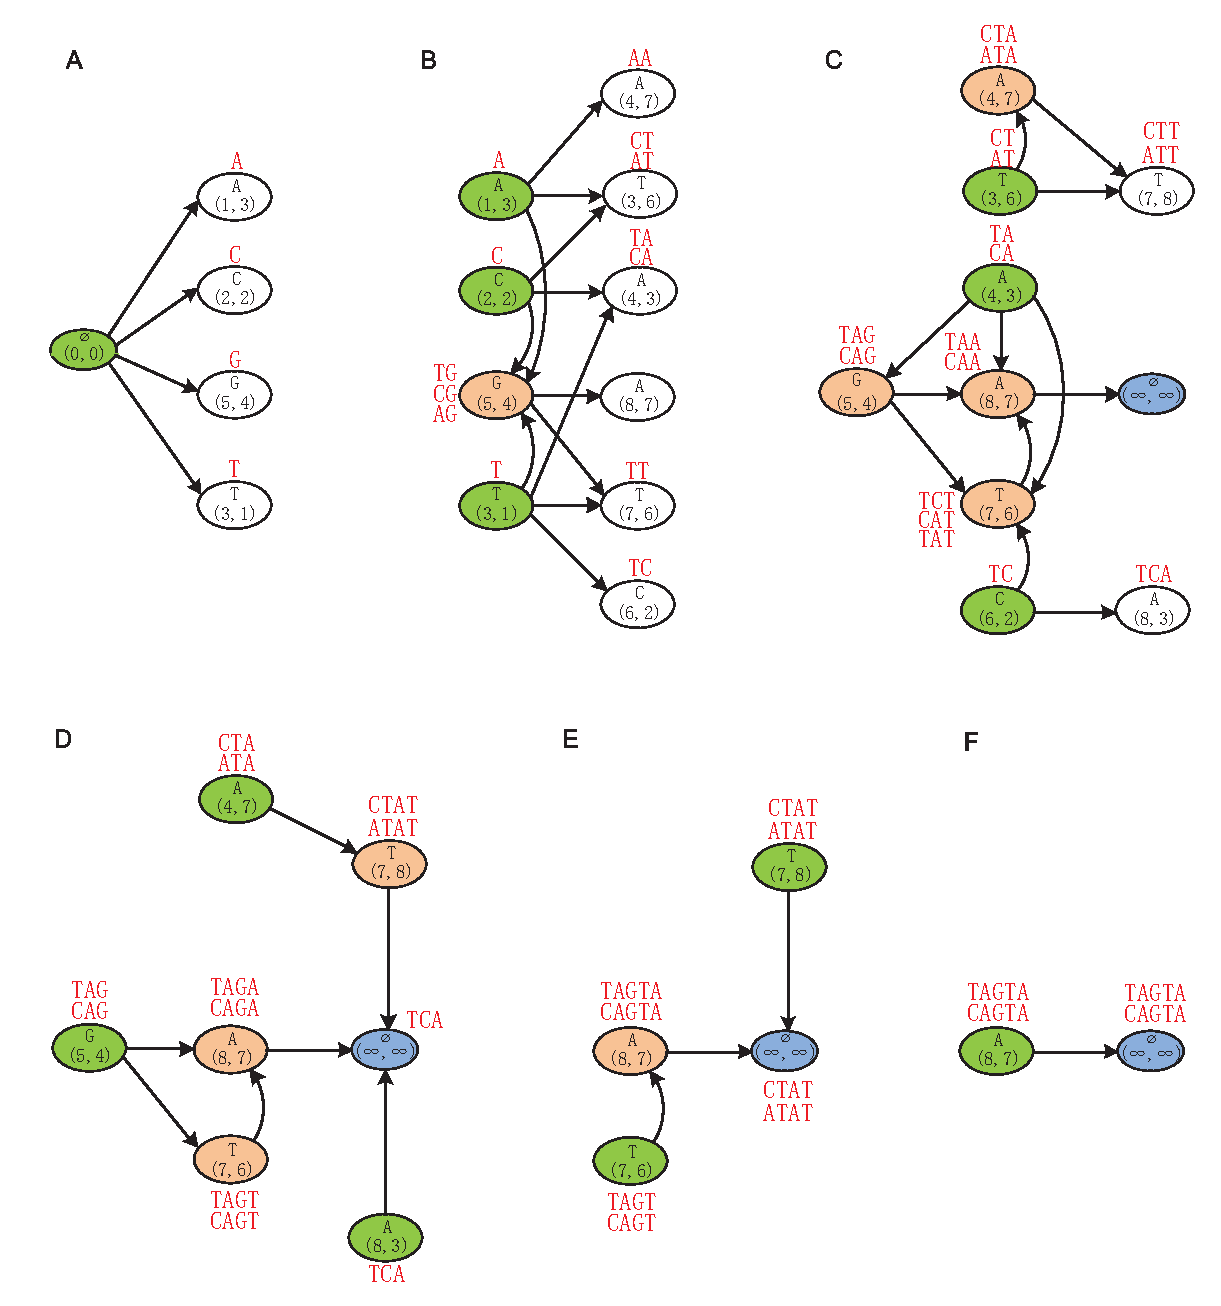
\includegraphics[height=4.5in, width=4.5in]{./eps/Level_DAG}
  \caption{序列 ACTAGCTA 和 TCAGGTAT 所对应的 Leveled-DAG. 匹配点及其对应字符在节
    点内部显示。 The partial LCSs are shown by red strings near the nodes. The
    white nodes are newly created and will be expanded later. The green ones are
    outdated and will be removed right away. The red ones with incoming edges
    are left from the previous levels and cannot be removed at present.}
  \label{fig:Leveled-DAG}
\end{figure}

\textbf{例 2.} 基于Leveled-DAG模型求解序列 $ACTAGCTA$ 和 $TCAGGTAT$ 的最长公共子
序列。 最初, Leveled-DAG只包含属于第0层的源节点 $(0, 0)$. 然后,通过查询
图\ref{fig:ST}中所示的后继表,产生源节点的4个后继: $A(1, 3)$, $C(2, 2)$, $G(5,
4)$和 $T(3, 1)$. 由于这4个后继属于第1层,它们的前缀序列分别是单个字符:$A$, $C$,
$G$ 和 $T$, 如图\ref{fig:Leveled-DAG} A 中对应节点上方的红色字符所示。 此时,由于
源节点入度为0,它已经过时,可以从图中安全删除。

然后,产生第1层节点的后继以构成第2层节点,这些后继是: $A(4, 7)$, $T(3, 6)$,
$A(4, 3)$, $A(8, 7)$, $T(7, 6)$ 和 $C(6, 2)$, 如图 \ref{fig:Leveled-DAG} B 所
示。 注意,如果一个后继已经存在于Leveled-DAG中 (比如 $G(5, 4)$), 它无需再重复产
生。 当第2层节点被产生之后, 由于节点 $A(1, 3)$, $C(2, 2)$ 和 $T(3, 1)$ 入度为0,
它们已经过时并将被删除, 此时, 其所包含的前缀序列需要被其后继节点继承并延
长。 例如, 已经过时的节点 $A(1, 3)$ 有3个后继: $A(4, 7)$, $T(3, 6)$ 和 $G(5, 4)$
(它没有对应于字符 $C$ 的后继). 每一个后继都需要将其所对应的字符附加到 $A(1, 3)$
的前缀序列(即 $A$)之后, 然后将延长后的前缀序列保存为其自己的前缀序列。 具体地,
后继 $A(4, 7)$ 将 $A$ 附加到 $A$ 之后, 然后将 $AA$ 保存为自己的前缀序
列。 后继 $T(3, 6)$ 将 $T$ 附加到 $A$ 之后, 然后将 $AT$ 作为自己的前缀序列。 类似
地,后继 $G(5, 4)$ 将 $G$ 附加到 $A$ 之后, 将 $AG$ 作为自己的前缀序列。 注意, 由
于 $G(5, 4)$ 同时是这3个过时节点的后继, 它通过继承并延长这3个节点的前缀序列, 得
到了自己的3个前缀序列,分别是: $TG$, $CG$ 和 $AG$。 在移除过时节点之后,图中仅剩
余7个节点。

接下来, 如图 \ref{fig:Leveled-DAG} C 所示, 产生第2层所有节点的所有后继:$T(7,
8)$ 和 $A(8, 3)$ 构成图的第3层。 注意, 由于节点 $A(8, 7)$ 没有任何后继, 令终止节
点 $(\infty, \infty)$ 为其唯一后继。 在第3层构建完毕之后, 节点 $T(3, 6)$, $A(4,
3)$ 和 $C(6, 2)$ 已经过时。 在移除它们之前, 其所包含的前缀序列需要被其后继节点继
承并延长。 作为特例, 由于 $A(4, 7)$ 是过时节点 $T(3, 6)$ 的一个后继, $T(3, 6)$ 的
前缀序列 $CT$ 和 $AT$, 将由 $A(4, 7)$ 继承并加以延长(附加 $A$)。 由于延长后的前
缀序列 $CTA$ 和 $ATA$ 比 $A(4, 7)$ 原有的前缀序列 $AA$ 要长, $A(4, 7)$ 的前缀序
列将被相应地更新为 $CTA$ 和 $ATA$。 类似地, 节点 $G(5, 4)$ 和 $T(7, 6)$ 的前缀序
列同样通过继承并延长其过时前驱的前缀序列加以更新。

如图 \ref{fig:Leveled-DAG} D 所示, 需要扩展新产生的第3层中的节点 $T(7,
8)$ 和 $A(8, 3)$。 由于这两个节点均没有后继, 终止节点将被定义为这两个节点的唯一
后继。 由于没有新的节点产生, 此后将不再需要扩展任何节点。 从此刻起,算法只需要不
断地删除过时节点,并更新其相应后继节点的前缀序列。 当前, 节点 $A(4, 7)$, $G(5,
4)$ 和 $A(8, 3)$ 将被移除。 通过继承 $A(8, 3)$ 的前缀序列 $TCA$, 终止节点将其作
为自身的前缀序列 (终止节点不附加任何字符)。 接着, 如图 \ref{fig:Leveled-DAG} E 所
示, 节点 $T(7, 6)$ 和 $T(7, 8)$ 将被移除, 相应地,终止节点的前缀序列将被更新
为 $CTAT$ 和 $ATAT$. 最终, 如图 \ref{fig:Leveled-DAG} F 所示, 在移除最后一个过时
节点 $A(8, 7)$ 之后, 终止节点的前缀序列会被更新为 $TAGTA$ 和 $CAGTA$, 它们即是输
入序列的最长公共子序列。

从以上例子可以看到, 最初仅有一个源节点存在于Leveled-DAG中, 然后节点的数量将不断增
加, 一旦不再有新的节点产生, 节点的数量将开始下降直到剩余终止节点。 在此过程中, 只
有新产生的节点和以前产生的入度不为0的节点会被保留在Leveled-DAG中, 极大地减少了存
储开销。 当Leveled-DAG构建结束后, 输入序列的最长公共子序列立即可得。

\subsection{Leveled-DAG 模型的构建算法 }
\label{sec:PMA}

本节将给出Leveled-DAG模型构建算法的形式化描述。

\textbf{算法 2. 构建 Leveled-DAG}
\begin{itemize}
\item \textbf{步骤 0.} 预处理。 对每一个输入序列,构造其后继表。
\item \textbf{步骤 1.} 构建Leveled-DAG的第一层。通过查询后继表产生源节点的所有后
  继,作为图的第一层。 令每一个后继所对应的字符作为其(单字符)前缀序列。删除源节
  点。
\item \textbf{步骤 2.} 产生Leveled-DAG的下一层节点并删除过时节
  点 (即“产生-删除”策略)。 如果在Leveled-DAG中存在未扩展节点, 则重复以下两个子
  步骤:
  \begin{itemize}
  \item \textbf{步骤 2.1(产生).} 对每一个未扩展节点 $t$, 产生 $t$ 的所有后继 (如果某个
    后继已经存在于图中,无需重复产生, 只需通过指针建立其与 $t$ 的后继关系)。 如
    果 $t$ 没有后继,令终止节点作为其唯一后继。
  \item \textbf{步骤 2.2 (删除).} 令 $|p|$ 表示节点 $p$ 所包含前缀序列的长度。 对每一个
    入度为0的节点 $p$, 以及 $p$ 的每一个后继 $s$:
    \begin{itemize}
    \item 如果 $|p| \geq |s|$, 则删除 $s$ 原有的前缀序列。 将 $s$ 所对应的字符附
      加到 $p$ 的每一个前缀系列之后, 将这些延长后的前缀序列作为 $s$ 的(新的)前缀
      序列加以保存。
    \item 否则,如果 $|p| = |s|-1$, 则将 $s$ 所对应的字符附加到 $p$ 的每一个前缀
      系列之后, 并将这些延长后的前缀序列添加到 $s$ 原有的前缀序列集中。
    \end{itemize}
    删除节点 $p$ 及其前缀序列集。
  \end{itemize}
\item \textbf{步骤 3.} 重复执行步骤 2.2, 直到剩余终止节点。
\item \textbf{步骤 4.} 输出终止节点所保存的前缀序列,即输入序列的最长公共子序列。
\end{itemize}

如算法 2 中所示, 在预处理 (步骤 0) 之后, Leveled-DAG最初只包含源节点(步骤 1), 然
后它采用 ”产生-删除“ 策略来产生下一层节点 (步骤 2.1) 和删除过时节
点 (步骤 2.2), 一旦Leveled-DAG中所有的节点都被扩展, 即不再有新节点产生, 算法开始
重复地删除过时节点 (步骤 3), 直到剩余终止节点。 最后, 输出终止节点所保存的前缀序
列,即输入序列的最长公共子序列(步骤 4)。

如下是算法2的伪代码描述, 其中所用到的数据结构在 \ref{sec:data structures} 节已经
介绍, 构造后继表的过程已经省略, 后继表被直接作为输入数据。 算法2中的步骤1和步
骤2被合并为一个 \emph{while} 循环 (7 $\sim$ 22行), 步骤3对应于随后
的 \emph{while} 循环 (24 $\sim$ 26行). 移除过时节点的操作被单独封装为一个函
数 $Remove\_Outdated$, 对应于 30 $\sim$ 49 行。

\begin{varalgorithm}{2:}
  \caption{伪代码}
  \footnotesize
  \label{alg:PMA}
  \begin{algorithmic}[1]
    \REQUIRE ~~\\
    输入序列的后继表.\\
    \ENSURE ~~\\
    输入序列的最长公共子序列.
    \STATE
    \STATE $Suc(source) \leftarrow \emptyset$, $P\_LCS(source) \leftarrow \emptyset$
    \STATE $Suc(end) \leftarrow \emptyset$, $P\_LCS(end) \leftarrow \emptyset$
    \STATE $L\_DAG \leftarrow \{source, end\}$
    \STATE $Cur\_Level \leftarrow \{source\}$
    \STATE
    \WHILE{$Cur\_Level \neq \emptyset$}
    \FOR {每一个节点 $t \in Cur\_Level$}
    \FOR {$t$ 的每一个后继 $s$}
    \STATE $Suc(t) \leftarrow Suc(t) \cup \{s\}$
    \IF{$s \notin L\_DAG$}
    \STATE $L\_DAG \leftarrow L\_DAG \cup \{s\}$
    \STATE $Next\_Level \leftarrow Next\_Level \cup \{s\}$
    \ENDIF
    \ENDFOR
    \IF{$t$ 没有后继}
    \STATE $Suc(t) \leftarrow \{end\}$
    \ENDIF
    \ENDFOR
    \STATE $Remove\_Outdated(L\_DAG)$
    \STATE $Cur\_Level \leftarrow Next\_Level$
    \ENDWHILE
    \STATE
    \WHILE {$\exists t \in L\_DAG$ and $t \neq end$}
    \STATE $Remove\_Outdated(L\_DAG)$
    \ENDWHILE
    \STATE
    \STATE 输出: $P\_LCS(end)$
    \STATE
    \STATE $Remove\_Outdated(L\_DAG):$
    \FOR {每一个入度为零的节点 $p \in L\_DAG$}
    \FOR {$p$ 的每一个后继 $s$}
    \STATE $|p| \leftarrow $ $p$ 所包含前缀序列的长度
    \STATE $|s| \leftarrow $ $s$ 所包含前缀序列的长度
    \STATE $\delta \leftarrow $ 节点 $s$ 所对应的字符
    \IF {$|p| \geq |s|$}
    \FOR {每一个 $plcs \in P\_LCS(p)$}
    \STATE 将 $\delta$ 附加到 $plcs$ 末尾
    \ENDFOR
    \STATE $P\_LCS(s) \leftarrow $ \{所有延长后的前缀序列\} 
    \ELSIF {$|p| + 1 = |s|$}
    \FOR {每一个 $plcs \in P\_LCS(p)$}
    \STATE 将 $\delta$ 附加到 $plcs$ 末尾
    \ENDFOR
    \STATE $P\_LCS(s) \leftarrow P\_LCS(s) \cup \{$所有延长后的前缀序列$\}$
    \ENDIF
    \STATE 从 $L\_DAG$ 中删除 $p$
    \ENDFOR
    \ENDFOR
  \end{algorithmic}
\end{varalgorithm}

\subsubsection{时间/空间复杂度分析}
\label{sec:complexity}

接下来将给出Leveled-DAG方法粗略的时间/空间复杂度分析。

如上所述, Leveled-DAG方法包含两个阶段: 1. 为每一个输入序列构造后继表; 2.基于后继
表构造Leveled-DAG图。 第一个阶段, 如 \ref{sec:successor table} 节所示, 对长为
$n$ 的序列,构造其后继表将花费 $O(|\Sigma|n)$ 时间, 因此,为 $d$ 个长为 $n$ 的序
列构造后继表将花费 $O(d|\Sigma|n)$ 时间。 对于第二个阶段, 从宏观角度来看, 构造
Leveled-DAG 图的过程仅仅是产生出所有图节点然后再将其全部删除 (除了终止节点)。 尽
管产生节点和删除节点在构建过程中交织在一起, 图中任意节点仅被产生并删除一次, 并且
整个构建过程不含任何递归调用 (见算法2的伪代码描述)。 因此, 构建图的时间复杂度为
$O(2|Nodes|)$, 其中 $|Nodes|$ 为产生的节点数量, 产生节点和删除节点的过程都需要
$O(|Nodes|)$ 时间。 结合这两个阶段, Leveled-DAG方法的时间复杂度为 $O(d|\Sigma|n
+ 2|Nodes|)$. 由于总是有 $O(d|\Sigma|n) \ll O(2|Nodes|)$ (由实验证实), 所以
$O(d|\Sigma|n + 2|Nodes|) \thickapprox O(2|Nodes|) \thickapprox O(|Nodes|)$, 这
意味着Leveled-DAG方法的时间复杂度与图中节点的数量呈线性关系。

对于空间复杂度, 一方面, Leveled-DAG 方法需要存储所有的后继表,这需
要 $O(d|\Sigma|(n+1))$ 的存储空间。 另一方面, 如前所述, Leveled-DAG 图主要需要保
存最新产生的一层节点, 且最新一层节点的数量会先增后降, 因此Leveled-DAG方法的内存开
销也会先增后降。 所以, Leveled-DAG方法的峰值内存消耗
为 $O(|Max\_Level|)$, 其中 $|Max\_Level|$ 是图中最大一层所包含节点的数量。 结合两
方面内存开销, Leveled-DAG方法的空间复杂度为 $O(d|\Sigma|(n+1) + |Max\_Level|)$,
由于总是有 $O(d|\Sigma|(n+1)) \ll O(|Max\_Level|)$, 所以
$O(d|\Sigma|(n+1) + |Max\_Level|) \thickapprox O(|Max\_Level|)$, 这意味
着Leveled-DAG方法的空间复杂度主要取决于图中最大一层的节点数量。


\section{实验及结果分析}
\label{sec:experiments}

本节将使用真实的生物序列,从时间和空间两方面来比较Leveled-DAG方法和其它三个主
流MLCS算法: \emph{Top\_MLCS} \cite{Li2016_ICDE}, \emph{Quick-DP}
\cite{Wang2011} 和 \emph{Fast\_LCS} \cite{Chen2006} 的性能。

\subsection{实验设定}
\label{Test problems}

实验将使用两种类型的生物序列: DNA序列 ($|\Sigma|=4$) 和蛋白质序
列 ($|\Sigma|=20$) 作为输入数据。 我们将进行两方面的实验:

\begin{enumerate}
\item 测试不同数量的序列: 对每一种类型的生物序列, 序列的长度固定为100,数量由3逐
  步增加到700.
\item 测试不同长度的序列: 对每一种类型的生物序列, 序列的数量固定为5个,长度由50逐
  步增加到5000.
\end{enumerate}

对每次实验, 根据指定的长度和数量,输入序列由一个大的原始序列集中随机抽取而产
生。 所有测试算法均由C/C++实现,由gcc编译器编译(-O2), 在同一台服务器上运行,配置
为: Intel Xeon E7-8880 2.2 GHz CPU, 700 GB内存 (由于服务器被多个用户共享,分配给
每个进程的内存被限定为300GB)。操作系统为 GNU/Linux (amd64).

\subsection{测试不同数量的序列}
\label{sec:number}

在第一种实验中,所有输入序列的长度均被固定为100, 序列的数量由3逐渐增加到700. 将
对DNA和蛋白质两种序列分别进行实验。 所有算法独立运行5次,使用32个线程,它们的平
均CPU占用时间(以及运行时间的标准差)和内存消耗被测量并分别显示于
表 \ref{tab:times1} 和表 \ref{tab:memory1} 中。 值得指出的是, 算法的运行时间和内
存消耗高度依赖于序列本身, 即使两个序列集包含相同数量和长度的序列, 如果其包含序列
本身不同, 算法在这两个序列集上的运行时间和内存消耗可能变化很大。

实验结果显示, 由于内存溢出,\emph{FAST\_LCS} 和 \emph{Quick-DP} 算法无法处理包
含20个或更多序列的序列集。 如表 \ref{tab:memory1} 所示, 这两个算法的内存占用相当
接近 (因为它们采用了同样的框架,唯一不同之处在于删除非支配节点的方式), 并且都随着
序列数量的增加呈指数增长, 这是因为二者都需要产生大量的冗余节点,并将其保存在内存
中。 如表 \ref{tab:times1} 所示, 它们的运行时间也随着序列数量的增长而快速增长,这
是因为随着序列个数的增加,每个节点所包含的匹配点的维数也相应增加。 因此, 为了删除
非支配节点, 两个算法所使用的 \emph{Minima} 操作需要在每一层中对所有节点的匹配向量
进行逐维度比较。 这需要大量的比较操作且非常耗时。 另一方面, \emph{Quick-DP} 相比
较 \emph{FAST\_LCS} 要快很多,因为它采用了非常适于并行化的分而治之的策略来删除非
支配点。 遗憾的是, \emph{Quick-DP} 算法在应对包含很多序列的序列集时,无论在时间或
空间方面仍然不够高效。

作为对比, 从试验结果可以看出 \emph{Top\_MLCS} 算法和本章提出
的 \emph{Leveled-DAG} 算法都可以处理高达 700 个序
列. 如表 \ref{tab:memory1} 所示, 二者的内存占用相比前两个算法都大幅减少, 这是因为
它们都采用了新的图模型来减小支配点图的规模: \emph{Top\_MLCS} 算法所用
的 \emph{ICSG} 模型不会产生冗余节点, 而 \emph{Leveled-DAG} 模型仅需要保存当前层及
以前层的一部分节点。 相比 \emph{Top\_MLCS}, \emph{Leveled-DAG} 算法对于(数量超
过100的)DNA和蛋白质序列,分别能够节省大约 $35\% \sim 40\%$ $/$ $33\% \sim 35\%$
的存储空间, 这是由于对于规模较大的序列集,Leveled-DAG所保存的(最大)节点数量(包括
最大一层的节点和以前层的入度非0的节点) 大约只占节点总数的 $40\%$。 需要注意的是,
起初两个算法的内存开销都会随着序列数量的增加而快速增长, 但是当序列数量增加到某个
特定值时 (本实验中,大约在 $80 \sim 90$ 之间), 算法的内存增长率开始降低, 且最终
算法的内存增长趋向一个常量。 我们发现,这是由于当序列的数量增长到某个特定的临界值
时,节点数量的增长率开始下降 (临界值非常难以确定,因为它由许多因素决定,比如序列
的字符集, 序列的长度和序列本身), 并且最终随着序列数量的进一步增长,图中的节点数量
将保持大致不变, 此时的空间增长主要来自于每个节点内部匹配点维数的增长。

时间方面, 两个算法比都比 \emph{FAST\_LCS} 和 \emph{Quick-DP} 算法快一到两个数量
级。 这主要是由于二者不需要类似于 \emph{FAST\_LCS} 和 \emph{Quick-DP} 算法所使用
的 \emph{Minima} 操作来. Compared with \emph{Top\_MLCS}, our \emph{Leveled-DAG}
is about $10\%$ faster for smaller datasets (containing less than 10 sequences),
and $10\%$ $\sim$ $20\%$ faster for larger datasets. This is because the
\emph{Top\_MLCS} algorithm needs two topological sorting operations (forward and
backward topological sort) to search for the MLCS after the graph is built,
while the \emph{Leveled-DAG} does not need any searching operation after
\emph{Leveled-DAG} is constructed. In fact, the wanted MLCS are saved in the
only end node left in the graph, which can be gotten immediately. This
demonstrates that the \emph{Leveled-DAG} approach is more suitable than the
compared algorithms for large-scale sequences sets. Note that, the growth in
running time of both algorithms also begins to slow down as the number of
sequences grows to a threshold.

From Table \ref{tab:times1} and Table \ref{tab:memory1}, we can also
see that both time and space efficiency of all the test algorithms for
protein sequences are superior to that for DNA sequences, this is
because the scale of DAG for large alphabet sequences (such as
protein) is smaller than that for small alphabet sequences (such as
DNA). We leave the detailed discussion of the effect of alphabet size
in the later section.


\subsection{Evaluation under various lengths of sequences}
\label{sec:times2}

In the second kind of experiment, each test is conducted on 5 DNA $/$ protein
sequences with length increasing from 50 to 5000. As before, all the algorithms
are independently run 5 times with 32 threads, and their average running times
(as well as the standard deviation of the running times) and memory consumption
are measured and shown in Table \ref{tab:times2} and Table \ref{tab:memory2},
respectively.

It can be seen from the experimental results that, the \emph{FAST\_LCS} cannot
process DNA sequences longer than 400 or protein sequences longer than 500 due
to the extremely long running time, while the \emph{Quick-DP} algorithm cannot
process DNA sequences longer than 800 or protein sequences longer than 1000 due
to out of memory. (Again, the performance of the algorithms for protein
sequences is better than that for DNA sequences). Since as the length of the
sequences increases, the number of levels in the graph will grow accordingly and
the nodes in each level will grow exponentially, which makes the graph take up
too much memory. Also, the running times of \emph{FAST\_LCS} and \emph{Quick-DP}
grow rapidly as the length of sequences increases, the main reason is that as
the nodes increase exponentially in each level, the \emph{Minima} operation for
the levels is very time-consuming, moreover searching the longest paths in a
graph with many levels is also time-consuming. Consequently, neither of the two
algorithms are suitable for finding MLCS of long sequences.

On the other hand, as shown in Table \ref{tab:memory2}, both
\emph{Top\_MLCS} and \emph{Leveled-DAG} can handle DNA$/$ protein
sequences with length up to 5000. Compared with \emph{Top\_MLCS}, the
\emph{Leveled-DAG} approach can save about $43\% \sim 46\%$ $/$
$41\% \sim 45\%$ of memory for DNA$/$protein sequences longer than
1000, since the growth in memory requirement of \emph{Leveled-DAG}
mainly depends on the max level of nodes, whose proportion in the
total nodes will decrease as the sequence length increases. Further,
as shown in Table \ref{tab:times2}, the running times of both
algorithms grow much more slowly than that of \emph{FAST\_LCS} and
\emph{Quick-DP}. Even for long sequences ($length \geq 1000$), both
\emph{Top\_MLCS} and \emph{Leveled-DAG} can still find their
MLCS. Particularly, note that in all cases, the proposed algorithm
\emph{Leveled-DAG} is the fastest algorithm: it is at least two orders
of magnitude faster than \emph{FAST\_LCS} and \emph{Quick-DP}, and
faster than \emph{Top\_MLCS} about $20\%$ on datasets with longer
sequences ($length \geq 2000$). The reason for the proposed algorithm
\emph{Leveled-DAG} being faster than \emph{Top\_MLCS} on longer
sequences is that with the increase of the length of sequences, the
first topological sorting scheme used in \emph{Top\_MLCS} will take
much more time, while the performance of \emph{Leveled-DAG} will not
be affected much by the sequence length. Thus \emph{Leveled-DAG}
algorithm is more suitable for finding MLCS of long sequences.

In general, due to the much smaller scale of the \emph{Leveled-DAG}
graph and the efficiency of the technique to gradually construct the
MLCS, the \emph{Leveled-DAG} approach has better performance than the
compared algorithms on all the testing datasets, especially on
datasets with long sequences and many sequences.


\section{Discussion}

Next, we will discuss some factors that can affect the performance of
the MLCS algorithms.The \emph{length} of the sequences is the key
factor that affects the performance of the algorithms: for the same
type of sequences, as the length of sequences increases, the number of
levels in the corresponding DAG will increase accordingly. Since the
number of nodes in the levels will grow (nearly) exponentially as the
level increases, the total number of nodes in DAG will explode as the
sequence length increases, therefore, the scale of DAG for long
sequences is larger than that for short sequences. Consequently, both
time and space overhead for finding MLCS of long sequences are higher
than that for finding MLCS of short sequences. On the other hand, the
\emph{number} of sequences can also have an impact on the algorithms'
performance: as the number of sequences increases, the dimension of
match point in each node will grow accordingly, and therefore each
single node in DAG will take up more space, moreover, comparing two
match point will require more time. In addition, the number and length
of the sequences can also affect the result MLCS: obviously, the
longer the sequences are, the longer the result MLCS are; conversely,
the more the sequences there are, the shorter the result MLCS are.

From the experimental results, we can also find that, the alphabet
size can have a significant impact on the performance of the
algorithms. For sequences with large alphabet (such as protein
sequences), the performance of the algorithms is much better than that
for sequences with small alphabet (such as DNA sequences). This is
because that, for a fixed-length sequence, the larger the alphabet
size is, the less each symbol appears in that sequence, which means
for large alphabet sequences, the "distance" between one node and its
successors is large, therefore the DAG for large alphabet sequences
has less levels than that for small alphabet sequences. For instance,
with the sequence length fixed to 100, the DAG for DNA sequences has
about 30 levels, while the DAG for protein sequences has only about 10
levels. Although a certain level in DAG for protein sequences has more
nodes than the same level in DAG for DNA sequences (since one node in
DAG for protein sequences can have up to 20 successors, however, for
DNA sequences one node has at most 4 successors), the total number of
graph nodes for protein sequences is smaller than that for DNA
sequences. Therefore, the performance of algorithms for large alphabet
sequences is much better than that for small alphabet sequences.

By profiling the program, we find that the most time-consuming part of
the Leveled-DAG approach is the procedure of deleting the outdated
nodes (i.e, the $Remove\_Outdated(L\_DAG)$ routine in Algorithm 2,
which takes about $50\% \sim 60\%$ of the total running time),
particularly, the procedure of passing the partial LCSs of one node to
its successors. This procedure needs a lot of memory allocation,
resize, and free operations, which is not appropriate for
parallelization and therefore very time-consuming. To reduce the time
consumption, we are focusing on more efficient passing strategy and
more carefully implementation. We are also searching for more
efficient memory management routines to replace the ones we used
(which are provided by the standard library).


\section{Conclusion}
\label{sec:conclusion}

In this paper, we propose a novel graph model called Leveled-DAG which
is much smaller than the existing DAG model. Based on this model, the
corresponding construction algorithm is also proposed. Once the
Leveled-DAG is constructed, there is only one node left with all MLCS
being immediately obtained without any further operation for searching
the MLCS. The experimental results also show the proposed approach is
both time and space efficient on all testing cases, especially for
long and large-scale sequences.

\section*{Conflict of Interest Statement}
% All financial, commercial or other relationships that might be
% perceived by the academic community as representing a potential
% conflict of interest must be disclosed. If no such relationship
% exists, authors will be asked to confirm the following statement:

The authors declare that the research was conducted in the absence of
any commercial or financial relationships that could be construed as a
potential conflict of interest.

\section*{Author Contributions}

Zhan Peng designs and implements the proposed algorithm. Zhan Peng
writes the initial manuscript, and Yuping Wang revises the manuscript.

\section*{Funding}

This work is supported by National Natural Science Foundation of China
(No.61472297).


\begin{table*}[htp]
  \footnotesize
  \caption{The average running times (in seconds) of the test
    algorithms on different numbers of DNA and protein sequences with
    the length of sequences fixed to 100.(Using 32 threads). The
    standard deviations of the running times are shown in the
    parentheses.}
  \label{tab:times1}
\resizebox{7in}{!}{
  \begin{tabular}{|r|r|r|r|r|r|r|r|r|r|}
    \hline
    Number &
    \multicolumn{4}{c|}{DNA ($|\Sigma|=4$)} & \multicolumn{4}{c|}{Protein ($|\Sigma|=20$)}\\
    \cline{2-9}
      & FAST\_LCS & Quick-DP & Top\_MLCS & Leveled-DAG & FAST\_LCS & Quick-DP & Top\_MLCS & Leveled-DAG \\
    \hline
    3  & 0.052 (0.003)    & 0.041 (0.001)  & 0.031 (0.002)  & 0.018 (0.001)  & 0.021 (0.001)    & 0.034 (0.002)  & 0.027 (0.001)  & 0.016 (0.001) \\
    4  & 0.255 (0.01)     & 0.203 (0.02)   & 0.071 (0.004)  & 0.053 (0.003)  & 0.183 (0.02)     & 0.152 (0.03)   & 0.051 (0.003)  & 0.037 (0.002) \\
    5  & 2.9 (0.1)        & 1.5 (0.09)     & 0.12 (0.008)   & 0.082 (0.004)  & 2.1 (0.1)        & 1.0 (0.08)     & 0.098 (0.008)  & 0.077 (0.006) \\
    6  & 26.5 (1.7)       & 10.3 (0.8)     & 1.3 (0.09)     & 1.1 (0.1)      & 20.8 (1.2)       & 6.9 (0.6)      & 0.94 (0.03)    & 0.75 (0.02)  \\
    7  & 151.8 (10.0)     & 32.8 (1.9)     & 3.6 (0.1)      & 2.7 (0.2)      & 116.5 (10.3)     & 21.8 (1.3)     & 2.8 (0.2)      & 1.9 (0.1) \\
    8  & 834.9 (43.8)     & 147.6 (8.8)    & 8.5 (0.6)      & 6.9 (0.4)      & 746.5 (58.8)     & 107.0 (8.7)    & 6.3 (0.3)      & 4.7 (0.2) \\
    9  & 4174.6 (408.7)   & 738.5 (51.5)   & 16.4 (0.9)     & 13.7 (0.6)     & 3059.2 (301.4)   & 585.6 (40.2)   & 12.5 (0.8)     & 9.9 (0.4) \\
                                                                                                                                  
    10 & 25671.4 (2433.8) & 3385.4 (326.4) & 30.0 (2.3)     & 25.3 (0.9)     & 22751.9 (1596.7) & 2645.3 (215.7) & 24.7 (1.5)     & 20.6 (1.1)  \\
    20 & --               & --             & 64.8 (4.6)     & 51.2 (2.1)     &  --              &  --            & 57.7 (3.3)     & 45.3 (2.3)  \\
    30 & --               & --             & 136.7 (6.7)    & 96.7 (3.7)     &  --              &  --            & 124.3 (8.9)    & 89.2 (4.7)  \\
    40 & --               & --             & 250.3 (9.4)    & 191.4 (7.5)    &  --              &  --            & 223.4 (14.7)   & 180.8 (10.5) \\
    50 & --               & --             & 463.2 (17.5)   & 380.1 (12.3)   &  --              &  --            & 432.7 (22.4)   & 366.4 (16.0) \\
    60 & --               & --             & 665.4 (42.2)   & 530.3 (27.4)   &  --              &  --            & 590.6 (31.2)   & 509.5 (20.4) \\
    70 & --               & --             & 1088.1 (76.7)  & 875.5 (39.4)   &  --              &  --            & 967.8 (76.4)   & 848.6 (39.6) \\
    80 & --               & --             & 1684.6 (127.5) & 1233.2 (62.3)  &  --              &  --            & 1432.6 (105.2) & 1167.0 (66.8) \\
    90 & --               & --             & 2217.9 (188.3) & 1764.6 (85.5)  &  --              &  --            & 2053.5 (127.1) & 1715.1 (84.1) \\
                                                                                                                                  
    100& --               & --             & 3041.5 (220.9) & 2417.8 (174.9) &  --              &  --            & 2320.2 (144.8) & 2056.2 (101.5)\\
    200& --               & --             & 3398.3 (241.4) & 2778.2 (190.2) &  --              &  --            & 2492.6 (152.4) & 2118.5 (114.9) \\
    300& --               & --             & 3665.0 (263.8) & 2962.5 (206.7) &  --              &  --            & 2614.2 (165.7) & 2214.3 (138.8) \\
    400& --               & --             & 3981.6 (285.0) & 3191.2 (218.0) &  --              &  --            & 2745.3 (172.8) & 2375.4 (152.9) \\
    500& --               & --             & 4237.2 (310.3) & 3384.0 (231.4) &  --              &  --            & 2862.4 (181.1) & 2435.1 (164.3) \\
    600& --               & --             & 4555.9 (336.9) & 3547.2 (243.7) &  --              &  --            & 2947.9 (193.4) & 2479.2 (170.7)\\
    700& --               & --             & 4880.3 (362.7) & 3854.7 (266.2) &  --              &  --            & 3174.8 (204.5) & 2511.9 (183.2)\\
    \hline
  \end{tabular}
  }
\end{table*}

\begin{table*}[htp]
  \footnotesize
  \caption{The memory consumption (in MB) of the test algorithms on
    different numbers of DNA and protein sequences with the length of
    sequences fixed to 100.}
  \label{tab:memory1}
 \begin{tabular}{|r|r|r|r|r|r|r|r|r|r|}
   \hline
   Number &
   \multicolumn{4}{c|}{DNA ($|\Sigma|=4$)} & \multicolumn{4}{c|}{Protein ($|\Sigma|=20$)}\\
   \cline{2-9}
     & FAST\_LCS & Quick-DP & Top\_MLCS & Leveled-DAG & FAST\_LCS & Quick-DP & Top\_MLCS & Leveled-DAG \\
   \hline
   3  & 28      & 31      &  8        & 5      & 25     & 28    & 7      & 4   \\
   4  & 373     & 447     &  23       & 17     & 330    & 403   & 19     & 14  \\
   5  & 1358    & 1485    &  93       & 85     & 1167   & 1304  & 77     & 62  \\
   6  & 3315    & 3490    &  297      & 223    & 2718   & 2960  & 203    & 190 \\
   7  & 5190    & 5862    &  534      & 489    & 4152   & 4706  & 469    & 418 \\
   8  & 11057   & 12051   &  1211     & 1124   & 8513   & 9871  & 1017   & 943 \\
   9  & 20634   & 21183   &  3058     & 2765   & 15138  & 16062 & 2538   & 2238\\

   10 & 35769   & 36934   &  5813     & 5232   & 25637  & 26048 & 4766   & 4251  \\
   20 & --      & --      &  32329    & 28126  &  --    &  --   & 24246  & 18045 \\
   30 & --      & --      &  48765    & 39291  &  --    &  --   & 36824  & 26713  \\
   40 & --      & --      &  67813    & 52607  &  --    &  --   & 49503  & 35182  \\
   50 & --      & --      &  91128    & 68103  &  --    &  --   & 64292  & 46137  \\
   60 & --      & --      &  121268   & 87359  &  --    &  --   & 81379  & 58174  \\
   70 & --      & --      &  156470   & 118600 &  --    &  --   & 98541  & 61036  \\
   80 & --      & --      &  197387   & 141859 &  --    &  --   & 117390 & 76283  \\
   90 & --      & --      &  209145   & 146402 &  --    &  --   & 120833 & 81429  \\


   100& --      & --      &  229372   & 151386 &  --    &  --   & 124124 & 84069  \\
   200& --      & --      &  252247   & 163948 &  --    &  --   & 131920 & 88132  \\
   300& --      & --      &  261963   & 167085 &  --    &  --   & 138255 & 92025  \\
   400& --      & --      &  268993   & 170811 &  --    &  --   & 144213 & 96044  \\
   500& --      & --      &  276103   & 173945 &  --    &  --   & 151318 & 101250 \\
   600& --      & --      &  290398   & 177140 &  --    &  --   & 157986 & 104986 \\
   700& --      & --      &  299498   & 179846 &  --    &  --   & 162298 & 108107 \\
   \hline
  \end{tabular}
\end{table*}





\begin{table*}[htp]
  \footnotesize
  \caption{The average running times of the test algorithms under
    different lengths of DNA and protein sequences with the number of
    sequences fixed to 5. (Using 32 threads). The standard deviations
    of the running times are shown in the parentheses.}
  \label{tab:times2}
  \resizebox{7in}{!}{
  \begin{tabular}{|r|r|r|r|r|r|r|r|r|r|}
     \hline
    Length &
    \multicolumn{4}{c|}{DNA ($|\Sigma|=4$)} & \multicolumn{4}{c|}{Protein ($|\Sigma|=20$)}\\
    \cline{2-9}
     & FAST\_LCS & Quick-DP & Top\_MLCS & Leveled-DAG & FAST\_LCS & Quick-DP & Top\_MLCS & Leveled-DAG \\
    \hline
    50   & 0.57 (0.03)   & 0.13 (0.01)     & 0.038 (0.002)   & 0.026 (0.001)    & 0.06 (0.001)   & 0.018 (0.001)    & 0.004 (0)     & 0.001 (0) \\
    100  & 2.7 (0.2)     & 1.4 (0.08)      & 0.23 (0.03)     & 0.96 (0.04)      & 0.3 (0.02)     & 0.16 (0.01)      & 0.077 (0.003) & 0.058 (0.006)\\
    200  & 244.1 (10.4)  & 10.6 (0.2)      & 8.5 (0.3)       & 6.8 (0.2)        & 28.5 (1.5)     & 1.2 (0.1)        & 0.96 (0.102)  & 0.77 (0.05) \\
    300  & 4064.8 (312.6)& 95.3 (4.7)      & 38.7 (2.2)      & 32.6 (2.7)       & 467.1 (14.4)   & 11.4 (1.1)       & 4.4 (0.2)     & 3.1 (0.2) \\
    400  & --            & 312.4 (11.5)    & 77.8 (4.9)      & 59.5 (3.8)       & 3659.2 (363.8) & 36.7 (1.8)       & 8.9 (0.8)     & 7.2 (0.6)  \\
    500  & --            & 1566.9 (128.9)  & 132.6 (7.8)     & 112.2 (5.6)      & --             & 180 (6.2)        & 15.2 (1.1)    & 12.7 (0.9) \\
    600  & --            & 4384.1 (297.4)  & 201.1 (11.7)    & 165.3 (8.3)      & --             & 533.8 (19.4)     & 23.1 (2.0)    & 18.9 (1.0) \\
    700  & --            & 10347.5 (913.2) & 287.3 (12.1)    & 223.4 (10.1)     & --             & 1075.5 (32.7)    & 32.6 (2.5)    & 24.6 (1.03) \\
    800  & --            & 27489.2 (2351.3)& 373.2 (14.5)    & 313.8 (13.3)     & --             & 2958.1 (61.5)    & 43.9 (3.8)    & 35.3 (1.1) \\
    900  & --            & --              & 487.3 (21.6)    & 399.1 (15.5)     & --             & 6709.0 (221.2)   & 54.1 (4.2)    & 44.8 (1.2) \\
                                                                                                 
    1000 & --            & --              & 644.7 (29.3)    & 513.5 (19.8)     & --             & 11508.6 (1258.9) & 70.8 (5.7)    & 57.0 (1.8) \\
    2000 & --            & --              & 4240.5 (251.2)  & 3017.6 (87.2)    & --             & --               & 469.3 (13.7)  & 355.4 (10.2)\\
    3000 & --            & --              & 9915.1 (673.8)  & 7922.0 (297.3)   & --             & --               & 1168.5 (30.5) & 873.1 (22.4)\\
    4000 & --            & --              & 16963.4 (1553.3)& 13762.3 (1433.4) & --             & --               & 1843.0 (41.3) & 1532.5 (32.4) \\
    5000 & --            & --              & 24672.9 (2104.3)& 19074.7 (1658.1) & --             & --               & 2788.3 (55.6) & 2065.2 (46.3) \\
    \hline
  \end{tabular}
  }
\end{table*}

\begin{table*}[htp]
  \footnotesize
  \caption{The memory consumption (in MB) of the test algorithms under
    different lengths of DNA and protein sequences with the number of
    sequences fixed to 5.}
  \label{tab:memory2}
  \begin{tabular}{|r|r|r|r|r|r|r|r|r|r|}
     \hline
    Length &
    \multicolumn{4}{c|}{DNA ($|\Sigma|=4$)} & \multicolumn{4}{c|}{Protein ($|\Sigma|=20$)}\\
    \cline{2-9}
     & FAST\_LCS & Quick-DP & Top\_MLCS & Leveled-DAG & FAST\_LCS & Quick-DP & Top\_MLCS & Leveled-DAG \\
    \hline
    50   & 47     & 56      & 21      & 17      & 40      & 42       & 18     & 11     \\
    100  & 1352   & 1481    & 99      & 82      & 1163    & 1296     & 81     & 56     \\
    200  & 8331   & 8652    & 2353    & 1469    & 6249    & 7963     & 1894   & 988   \\
    300  & 16874  & 16993   & 4050    & 3051    & 11047   & 12735    & 3251   & 1864  \\
    400  & --     & 27355   & 5866    & 4787    & 113665  & 20586    & 4819   & 3012  \\
    500  & --     & 41257   & 8297    & 6654    & --      & 32771    & 6770   & 4351   \\
    600  & --     & 60912   & 12063   & 8598    & --      & 46009    & 9023   & 5806   \\
    700  & --     & 85733   & 18550   & 10163   & --      & 65574    & 11652  & 7513   \\
    800  & --     & 126483  & 26070   & 14250   & --      & 86684    & 14725  & 9426   \\
    900  & --     & --      & 36341   & 20539   & --      & 111748   & 18380  & 11573  \\

    1000 & --     & --      & 49442   & 27985   & --      & 140457   & 22507  & 13690  \\
    2000 & --     & --      & 95784   & 55549   & --      & --       & 45633  & 27811  \\
    3000 & --     & --      & 152178  & 86732   & --      & --       & 71058  & 42669  \\
    4000 & --     & --      & 224135  & 125454  & --      & --       & 99564  & 58937 \\
    5000 & --     & --      & 301375  & 165756  & --      & --       & 134568 & 77502 \\
    \hline
  \end{tabular}
\end{table*}




% for Science, Engineering and Humanities and Social Sciences
% articles, for Humanities and Social Sciences articles please include
% page numbers in the in-text citations
% \bibliographystyle{frontiersinHLTH&FPHY} % for Health, Physics and Mathematics articles

%%% Make sure to upload the bib file along with the tex file and PDF
%%% Please see the test.bib file for some examples of references

\bibliography{frontiers}
\bibliographystyle{frontiersinSCNS_ENG_HUMS}






%%% If you don't add the figures in the LaTeX files, please upload them when submitting the article.

%%% Frontiers will add the figures at the end of the provisional pdf automatically %%%

%%% The use of LaTeX coding to draw Diagrams/Figures/Structures should be avoided. They should be external callouts including graphics.

\end{document}

%%% Local Variables:
%%% mode: latex
%%% TeX-master: t
%%% End:

\message{ !name(ch_3.tex) !offset(-1021) }
